\section*{Appendix}

\subsection*{Site split formulation}

Since we have a finite character alphabet, for a given column $i$ there are a finite number of possible assignments of characters to tips $\alignmentColumn_i$ or internal nodes $\ancestralStateColumn_i$; this results in a simplification of likelihood calculation (we follow Section 8.6 of \cite{Semple2003-em}).
Take the tip labels of $\tau$ to be $\{1,\ldots,\nSiteRows\}$.
For likelihood calculation under the binary symmetric model, we describe a given $\alignmentColumn_i$ as a subset of indices $\siteSplit\subseteq\siteSplitSet:=\{1,\ldots,\nSiteRows-1\}$ with equivalent characters, commonly called a ``site split.''
Indeed, we start by including those tip labels in $\siteSplit$ that are assigned a 1 in the $\alignmentColumn_i$.
Then, because the probability of observing a particular collection of binary characters is equivalent to the probability of its complement under the binary symmetric model, we take the complement if needed to exclude label $\nSiteRows$ from $\siteSplit$.

For topology $\tau$, we define an ordered set of internal node labels $\{1,\ldots,\nAncestralStateRows\}$ for $\ancestralStateColumn_i$ and similarly use a subset of characters $\ancestralSplit\subseteq\ancestralSplitSet:=\{1,\ldots,\nAncestralStateRows\}$ to describe a realization of $\ancestralStateColumn_i$.
In this case the entire set of internal nodes must be enumerated: the probability of observing an ancestral state split, conditional on a site split, is not invariant to taking its complement.

We enumerate the site splits $\siteSplit_j$ of which there are $\nSiteSplits=|\mathcal{P}(\siteSplitSet)|$ in total where $\mathcal{P}$ denotes the power set.
Similarly we enumerate ancestral splits $\ancestralSplit_k$ of which there are $\nAncestralSplits=|\mathcal{P}(\ancestralSplitSet)|$ in total.

This split formulation defines mappings from patterns to splits as
 $$
 \patternToSplit:\alphabet^\nSiteRows\rightarrow\mathcal{P}(\siteSplitSet).
 $$
Given a site pattern--valued random variable $\alignmentColumnRV$, define the random variable
$$
\siteSplitRV := \patternToSplit(\alignmentColumnRV)
$$
that takes corresponding realizations $\siteSplit_j$ for some $j$.

For the $i$th factor of \eqref{eq:full_likelihood},
$$
P(\alignmentColumnRV=\alignmentColumn_i, \ancestralStateColumnRV=\ancestralStateColumn_i \mid \tau, t) = P(\alignmentColumnRV=\alignmentColumn_i \mid \tau, t) \cdot P(\ancestralStateColumnRV=\ancestralStateColumn_i \mid \alignmentColumnRV=\alignmentColumn_i, \tau, t).
$$
As a consequence of assuming a binary symmetric model, taking complements yields
\begin{align*}
    2\cdot P(\alignmentColumnRV=\alignmentColumn_i \mid \tau, t) &= P(\siteSplitRV=\patternToSplit(\alignmentColumn_i) \mid \tau, t) \\
                                                                 &= P(\siteSplitRV=\siteSplit_j \mid \tau, t)
\end{align*}
for some $j$.
For the other term, we define
$$
\ancestralToSplit:\alphabet^\nAncestralStateRows\times\alphabet^\nSiteRows\rightarrow\mathcal{P}(\ancestralSplitSet)
$$
as a mapping of ancestral states and tip states to ancestral state splits.
It is defined by whether the tip states have their complements taken or not: if a set of tip labels $\alignmentColumn$ is in $\siteSplitSet$, $\ancestralToSplit(\alignmentColumn, \ancestralStateColumn)$ is $\ancestralStateColumn$; otherwise, if $\alignmentColumn$ is not in $\siteSplitSet$, then the complement of $\alignmentColumn$ necessarily is in $\siteSplitSet$, and $\ancestralToSplit(\alignmentColumn, \ancestralStateColumn)$ is the complement of $\ancestralStateColumn$.
We define
$$
\ancestralSplitRV := \ancestralToSplit(\alignmentColumnRV, \ancestralStateColumnRV)
$$
for a tip state--valued random variable $\alignmentColumnRV$ and an ancestral state--valued random variable $\ancestralStateColumnRV$, so that
%By considering the case requiring complementing and that not requiring complementing separately,
%das: did I write the above? I don't remember the significance of it...
\begin{align*}
    P(\ancestralStateColumnRV=\ancestralStateColumn_i \mid \alignmentColumnRV=\alignmentColumn_i, \tau, t) &= P(\ancestralSplitRV=\ancestralToSplit(\alignmentColumn_i, \ancestralStateColumn_i) \mid \siteSplitRV=\patternToSplit(\alignmentColumn_i), \tau, t).
\end{align*}
Given $(\tau, t)$, there exists an ordered list of sets $\fullAncestralSplitPartitions(\tau, t)=(\ancestralSplitPartition_1(\tau, t),\ldots,\ancestralSplitPartition_\nSiteSplits(\tau, t))$ such that any element $\xi_j$ of the $j$th component $\ancestralSplitPartition_j(\tau, t)$ satisfies
\begin{align*}
\max_{\ancestralSplit_k\in\mathcal{P}(\ancestralSplitSet)} \ P(\ancestralSplitRV=\ancestralSplit_k \mid \siteSplitRV=\siteSplit_j, \tau, t) &= P(\ancestralSplitRV = \xi_j \mid \siteSplitRV=\siteSplit_j, \tau, t).
\end{align*}
In other words, for the $j$th site split, $\ancestralSplitPartition_j(\tau, t)\subset\mathcal{P}(\ancestralSplitSet)$ is the set of most likely ancestral splits for that particular site split, topology and set of branch lengths, and $\xi_j$ is one of possibly many equiprobable ancestral state splits in $\ancestralSplitPartition_j(\tau, t)$.
For each $\alignmentColumn_i$, $\ancestralToSplit(\alignmentColumn_i, \cdot)$ is surjective, and from this have
\begin{align*}
\max_{\ancestralStateColumn_i} P(\ancestralSplitRV=\ancestralToSplit(\alignmentColumn_i, \ancestralStateColumn_i) \mid \siteSplitRV=\patternToSplit(\alignmentColumn_i), \tau, t) &= P(\ancestralSplitRV = \xi_j \mid \siteSplitRV=\siteSplit_j, \tau, t).
\end{align*}

\subsection*{Site split likelihood}

Let $\xi_j$ be such a choice for each $1 \leq j \leq q$ in the following.
Then, the likelihood in \eqref{eq:profile_likelihood} written as a product over site patterns as opposed to sites is
\begin{align}
L_\nCols'(\tau, t; \fullAlignment) &= \max_{\fullAncestralStates} \ L_\nCols(\tau, t; \fullAlignment, \fullAncestralStates) \nonumber \\
                             &= \prod_{i=1}^{\nCols} \ \max_{\ancestralStateColumn_i} \ P(\alignmentColumnRV=\alignmentColumn_i, \ancestralStateColumnRV=\ancestralStateColumn_i \mid \tau, t) \nonumber \\
                             &\propto \prod_{i=1}^{\nCols} \ \max_{\ancestralStateColumn_i} \ P(\siteSplitRV=\patternToSplit(\alignmentColumn_i) \mid \tau, t) \cdot P(\ancestralSplitRV=\ancestralToSplit(\alignmentColumn_i, \ancestralStateColumn_i) \mid \siteSplitRV=\patternToSplit(\alignmentColumn_i), \tau, t) \nonumber \\
                             &= \prod_{i=1}^{\nCols} \ P(\siteSplitRV=\patternToSplit(\alignmentColumn_i) \mid \tau, t) \cdot \max_{\ancestralStateColumn_i} P(\ancestralSplitRV=\ancestralToSplit(\alignmentColumn_i, \ancestralStateColumn_i) \mid \siteSplitRV=\patternToSplit(\alignmentColumn_i), \tau, t) \nonumber \\
                             &= \prod_{j=1}^{\nSiteSplits} \ \left[P(\siteSplitRV=\siteSplit_j \mid \tau, t)\cdot P(\ancestralSplitRV=\xi_j \mid \siteSplitRV=\siteSplit_j, \tau, t)\right] ^{\nCols_j(\fullAlignment)} \label{eq:site_pattern_likelihood}
\end{align}
where $\nCols_j(\fullAlignment)$ is the number of columns in $\fullAlignment$ where the site split $\siteSplit_j$ or its complement appears.

Let
$$
L_\nCols''(\tau, t; \fullAlignment, \fullAncestralSplitPartitions(\tau, t)) = \prod_{j=1}^{\nSiteSplits} \ \left[P(\siteSplitRV=\siteSplit_j \mid \tau, t) \cdot P(\ancestralSplitRV=\xi_j \mid \siteSplitRV=\siteSplit_j, \tau, t)\right] ^{\nCols_j(\fullAlignment)}
$$
be the final product in \eqref{eq:site_pattern_likelihood}.
Assume $\nCols$ observations are generated from a model with parameters $(\tau^*, t^*)$.
We have
\begin{equation*}
\begin{split}
&    \frac{1}{\nCols} \log L_\nCols''(\tau, t; \fullAlignment, \fullAncestralSplitPartitions(\tau,t)) \\
&\qquad = \sum_{j=1}^\nSiteSplits \frac{\nCols_j(\fullAlignment)}{\nCols}\cdot  \log P(\siteSplitRV=\siteSplit_j, \ancestralSplitRV=\xi_j \mid \tau, t) \\
&\qquad = \sum_{j=1}^\nSiteSplits \frac{\nCols_j(\fullAlignment)}{\nCols}\cdot [\log P(\siteSplitRV=\siteSplit_j \mid \tau, t) +
            \log P(\ancestralSplitRV=\xi_j \mid \siteSplitRV=\siteSplit_j , \tau, t)]
\end{split}
\end{equation*}
so that, in the limit of infinite data,
\begin{equation}
\begin{split}
&    \frac{1}{\nCols} \log L_\nCols''(\tau, t; \fullAlignment, \fullAncestralSplitPartitions(\tau, t)) \\
&\qquad \rightarrow \sum_{j=1}^\nSiteSplits P(\siteSplitRV=\siteSplit_j \mid \tau^*, t^*) \cdot [\log P(\siteSplitRV=\siteSplit_j \mid \tau, t) + \log P(\ancestralSplitRV=\xi_j \mid \siteSplitRV=\siteSplit_j , \tau, t)]. \label{eq:site_pattern_profile_likelihood_mean}
\end{split}
\end{equation}
Define the divergence quantity
$$
\shannonDivergence_{\tau^*,t^*}(\tau,t) = \sum_{j=1}^\nSiteSplits P(\siteSplitRV=\siteSplit_j \mid \tau^*, t^*)\cdot\log P(\siteSplitRV=\siteSplit_j \mid \tau, t),
$$
and the partial log likelihood
$$
\tilde{\ell}_{\tau^*,t^*}(\tau, t; \fullAncestralSplitPartitions(\tau,t)) = \sum_{j=1}^\nSiteSplits P(\siteSplitRV=\siteSplit_j \mid \tau^*, t^*)\cdot\log P(\ancestralSplitRV=\xi_j \mid \siteSplitRV = \siteSplit_j, \tau, t)
$$
so that \eqref{eq:site_pattern_profile_likelihood_mean} becomes
\begin{equation}
    \label{eq:log_likelihood_simplified}
    \ell_{\tau^*,t^*}(\tau, t; \fullAncestralSplitPartitions(\tau,t)) = \shannonDivergence_{\tau^*,t^*}(\tau,t) + \tilde{\ell}_{\tau^*,t^*}(\tau, t; \fullAncestralSplitPartitions(\tau,t)).
\end{equation}

\subsection*{Hadamard transform}

Define: $\mathcal{T}$, $X$, $A$, $n$, $P$ and $\theta$.
Let
$$
\theta(e) = 1-2p(e).
$$
Then
\begin{equation}
\label{eq:hadamard_probability}
p_A = \frac{1}{2^{n-1}} \ \sum_{Y \subset X : |Y| \equiv 0 (\mathrm{mod} \ 2)} \ \left[(-1)^{|Y \cap A|} \ \prod_{e \in P(\mathcal{T}, Y)} \ \theta(e) \right]
\end{equation}

\paragraph{Example}
\begin{figure}
    \centering
    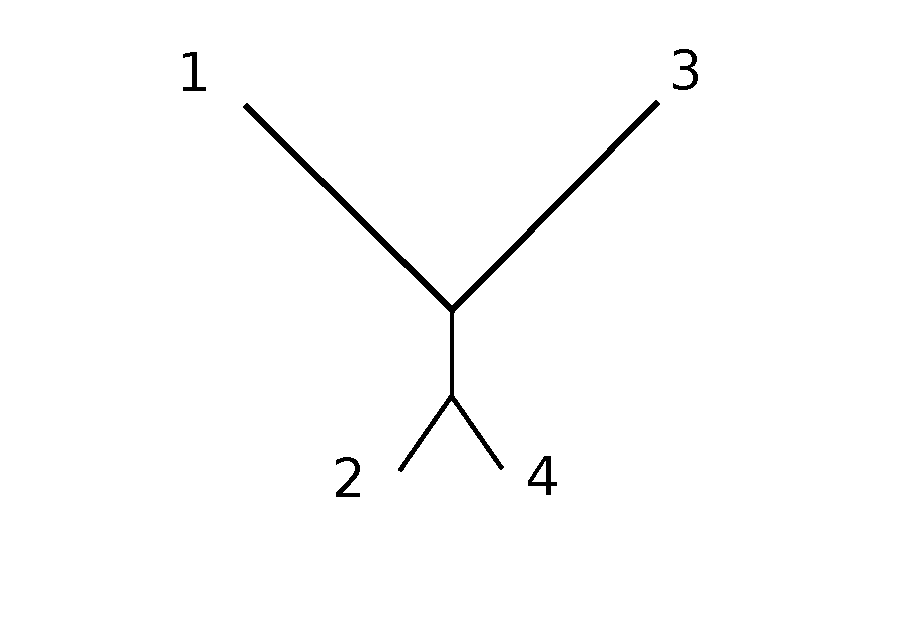
\includegraphics[width=.45\textwidth]{unrooted_farris_tree}
    \caption{Four taxon ``Farris zone'' tree.}
\label{fig:four-taxa-tree}
\end{figure}

Consider the fixed, binary four-tip tree $\tau$ in Fig.~\ref{fig:four-taxa-tree}---this is commonly known as the ``Farris zone'' topology.
The set of all possible character assignments is
\begin{align*}
\mathcal{P}(\{1,2,3,4\}) &= \{\emptyset, \{1,2,3,4\}, \{1\}, \{2,3,4\}, \{2\}, \{1,3,4\}, \{3\}, \{1,2,4\}, \\
                         &\qquad \{1,2\}, \{3,4\}, \{1,3\}, \{2,4\}, \{2,3\}, \{1,4\}, \{1,2,3\}, \{1,4\}\}.
\end{align*}
where each set indicates the tips assigned the character $1$.
For example, $\emptyset$ is the labeling $0000$ and $\{1,3,4\}$ is the labeling $1011$.
Symmetry allows us to group adjacent pairs in $\mathcal{P}(\{1,2,3,4\})$ into equiprobable splits, letting $\siteSplitSet=\{1,2,3\}$.
The unique site splits, collapsing complements, are
\begin{align*}
    \mathcal{P}(\siteSplitSet) &= \{\emptyset, \{1\}, \{2\}, \{3\}, \{1,2\}, \{1,3\}, \{2,3\}, \{1,2,3\}\} \\
& := \{\siteSplit_1, \ldots, \siteSplit_8\}.
\end{align*}
Since we identify character complements, we do not consider the additional splits
\begin{equation*}
\begin{split}
& \mathcal{P}(\{1,2,3,4\}) \setminus \mathcal{P}(\siteSplitSet) = \\
&\qquad \{\{1,2,3,4\}, \{2,3,4\}, \{1,3,4\}, \{1,2,4\}, \{3,4\}, \{2,4\}, \{1,4\}, \{4\}\},
\end{split}
\end{equation*}
the symmetry of the binary character model allowing us to focus only on the elements of $\mathcal{P}(\siteSplitSet)$.
This tree has two internal nodes with $\ancestralSplitSet=\{1,2\}$ and unique ancestral state splits
$$
\mathcal{P}(\ancestralSplitSet) = \{\emptyset, \{1\}, \{2\}, \{1,2\}\}.
$$
Internal node $\{1\}$ is the node connected to leaves $\{1\}$ and $\{3\}$ and internal node $\{2\}$ connected to leaves $\{2\}$ and $\{4\}$.
The mapping from characters to splits in this case will depend on the characters at the tips and the ancestral states.
For example, we take both $\patternToSplit(0000)=\emptyset$ and $\patternToSplit(1111)=\emptyset$.
Similarly, we have $\ancestralToSplit(0000, 00) = \emptyset$ and $\ancestralToSplit(1111, 11)=\emptyset$, needing to take the complement of all the characters present on the tree to identify splits.
We cannot identify complements for ancestral states in the same way as tip states since, for $\siteSplit\in\mathcal{P}(\siteSplitSet)$,
$$
P(\ancestralSplitRV=\emptyset \mid \siteSplitRV=\siteSplit, \tau, t)\neq P(\ancestralSplitRV=\{1,2\} \mid \siteSplitRV=\siteSplit, \tau, t)
$$
in general.

For each site split $\siteSplit\in\mathcal{P}(\siteSplitSet)$, we maximize the likelihood over all $\ancestralSplit\in\mathcal{P}(\ancestralSplitSet)$.
A maximum occurs at one of possibly several ancestral splits in $\mathcal{P}(\ancestralSplitSet)$, defined via $\ancestralSplitPartition_j(\tau, t)$ for the $j$th site split.
As a simple example, say all branch lengths correspond to a probability $p$ ($< 1/2$) of changing character along that branch.
The probabilities of observing ancestral splits for $\siteSplit_1=\emptyset$ are
$$
P(\ancestralSplitRV=\emptyset \mid \siteSplitRV=\emptyset, \tau, t) =
(1-p)^5,
$$
$$
P(\ancestralSplitRV=\{1\} \mid \siteSplitRV=\emptyset, \tau, t) =
P(\ancestralSplitRV=\{2\} \mid \siteSplitRV=\emptyset, \tau, t) =
p^3(1-p)^2,
$$
$$
P(\ancestralSplitRV=\{1,2\} \mid \siteSplitRV=\emptyset, \tau, t) =
p^4(1-p).
$$
The set of most likely ancestral states contains a single element, here $\ancestralSplitPartition_1(\tau, p)=\{\emptyset\}$.
Then, taking $\xi_1\in\ancestralSplitPartition_1(\tau, p)$ we have
$$
P(\ancestralSplitRV=\xi_1 \mid \siteSplitRV=\emptyset, \tau, t) =
P(\ancestralSplitRV=\emptyset \mid \siteSplitRV=\emptyset, \tau, t) =
(1-p)^5.
$$
For $\siteSplit_5=\{1,2\}$ we have
$$
P(\ancestralSplitRV=\emptyset \mid \siteSplitRV=\{1,2\}, \tau, t) =
P(\ancestralSplitRV=\{1,2\} \mid \siteSplitRV=\{1,2\}, \tau, t) =
p^2(1-p)^3,
$$
$$
P(\ancestralSplitRV=\{1\} \mid \siteSplitRV=\{1,2\}, \tau, t) =
P(\ancestralSplitRV=\{2\} \mid \siteSplitRV=\{1,2\}, \tau, t) =
p^3(1-p)^2.
$$
Here, the set of most likely ancestral states is $\ancestralSplitPartition_5(\tau, p)=\{\emptyset,\{1,2\}\}$, and, for $\xi_5\in\ancestralSplitPartition_5(\tau, p)$,
$$
P(\ancestralSplitRV=\xi_5 \mid \siteSplitRV=\{1,2\}, \tau, t) =
p^2(1-p)^3.
$$

\subsection*{Likelihood computations}

Table~\ref{tab:sitepatprob} contains calculations of site pattern frequencies under these two topologies.
Table~\ref{tab:likelihoods} contains calculations of likelihood values for fixed site patterns and topologies that have been maximized over ancestral state patterns.
Tables~\ref{tab:farris_likelihoods} and~\ref{tab:fels_likelihoods} contain the values of the likelihood for all possible ancestral states.

To compute the likelihood of observing a set of data, we need $P(\ancestralStateColumn=\ancestralSplit_k\mid \alignmentColumn=\siteSplit_j,\tau,t)$ for each $\ancestralSplit_k$ and $\siteSplit_j$.
The probability of a character change along a branch with fidelity parameter $x$ is $(1-x)/2$, while the probability of a character remaining the same is $(1+x)/2$.
See Fig.~\ref{fig:example_likelihoods} for the parameters on an example site pattern.
Likelihood computations for all site patterns and ancestral states are in Tables~\ref{tab:farris_likelihoods} and~\ref{tab:fels_likelihoods}.
Taking maxima row-wise of each table results in Table~\ref{tab:likelihoods}

\begin{figure}
\centering
\begin{subfigure}{.45\linewidth}
\centering
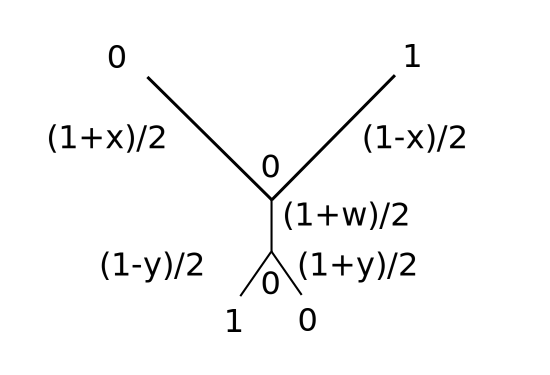
\includegraphics[width=.95\textwidth]{farris_like00}
\caption[short]{$P(\ancestralStateColumn=\emptyset\mid \alignmentColumn=\{2,3\},\tau_1,\{x,y,w\})$}
\end{subfigure}
\begin{subfigure}{.45\linewidth}
\centering
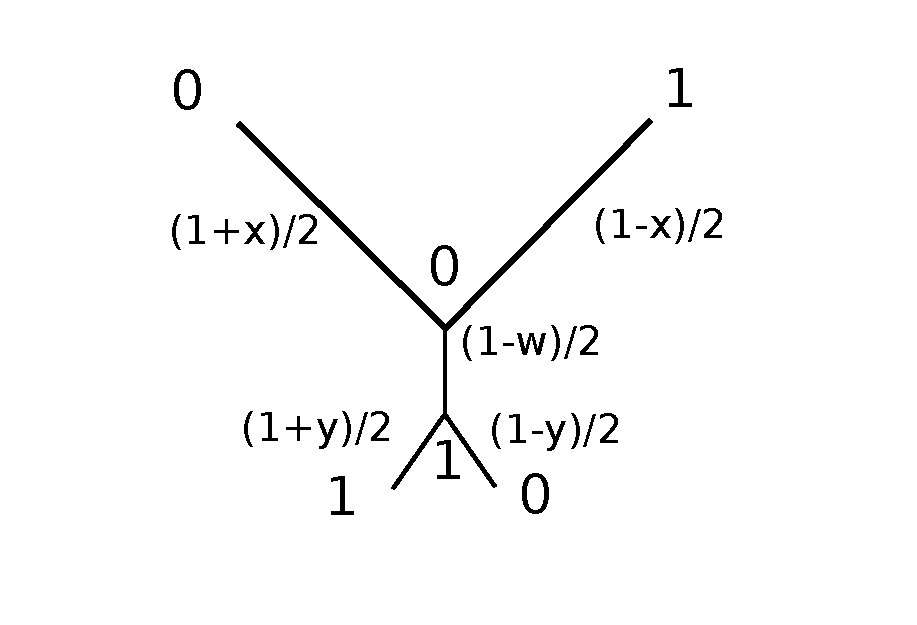
\includegraphics[width=.95\textwidth]{farris_like01}
\caption[short]{$P(\ancestralStateColumn=\{2\}\mid \alignmentColumn=\{2,3\},\tau_1,\{x,y,w\})$}
\end{subfigure}
\vskip\baselineskip
\begin{subfigure}{.45\linewidth}
\centering
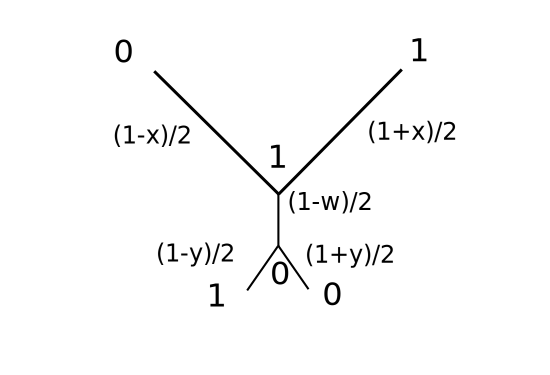
\includegraphics[width=.95\textwidth]{farris_like10}
\caption[short]{$P(\ancestralStateColumn=\{1\}\mid \alignmentColumn=\{2,3\},\tau_1,\{x,y,w\})$}
\end{subfigure}
\begin{subfigure}{.45\linewidth}
\centering
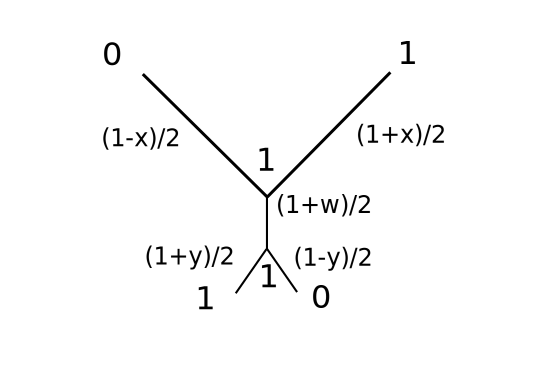
\includegraphics[width=.95\textwidth]{farris_like11}
\caption[short]{$P(\ancestralStateColumn=\{1,2\}\mid \alignmentColumn=\{2,3\},\tau_1,\{x,y,w\})$}
\end{subfigure}
\caption{Example likelihood computation}
\label{fig:example_likelihoods}
\end{figure}

\begin{table}
\centering
\begin{tabular}{|l|ll|}
\multicolumn{3}{c}{$P(\ancestralStateColumn=\ancestralSplit_k\mid \alignmentColumn=\siteSplit_j,\tau_1,t)$}\\
\hline
& \multicolumn{2}{|c|}{$\ancestralSplit_k$}\\
    \hline
    $\siteSplit_j$    &$\emptyset$                                &$\{2\}$  \\
    \hline
     $\emptyset$   &$(1+x)^2   (1+w)(1+y)^2$          &$(1+x)^2   (1-w)(1-y)^2$\\
     $\{1\}$       &$(1+x)(1-x)(1+w)(1+y)^2$          &$(1+x)(1-x)(1-w)(1-y)^2$\\
     $\{2\}$       &$(1+x)^2   (1+w)(1+y)(1-y)$       &$(1+x)^2   (1-w)(1+y)(1-y)$\\
     $\{3\}$       &$(1+x)(1-x)(1+w)(1+y)^2$          &$(1+x)(1-x)(1-w)(1-y)^2$\\
     $\{1,2\}$     &$(1+x)(1-x)(1+w)(1+y)(1-y)$       &$(1+x)(1-x)(1-w)(1+y)(1-y)$\\
     $\{1,3\}$     &$(1+x)^2   (1+w)(1-y)^2$          &$(1+x)^2   (1-w)(1+y)^2$\\
     $\{2,3\}$     &$(1+x)(1-x)(1+w)(1+y)(1-y)$       &$(1+x)(1-x)(1-w)(1+y)(1-y)$\\
     $\{1,2,3\}$   &$(1+x)^2   (1+w)(1+y)(1-y)$       &$(1+x)^2   (1-w)(1+y)(1-y)$\\
    \hline
    \hline
    &$\{1\}$                             &$\{1,2\}$  \\
    \hline
     $\emptyset$   &$(1-x)^2   (1-w)(1+y)^2$     &$(1-x)^2   (1+w)(1-y)^2$\\
     $\{1\}$       &$(1+x)(1-x)(1-w)(1+y)^2$     &$(1+x)(1-x)(1+w)(1-y)^2$\\
     $\{2\}$       &$(1-x)^2   (1-w)(1+y)(1-y)$  &$(1-x)^2   (1+w)(1+y)(1-y)$\\
     $\{3\}$       &$(1+x)(1-x)(1-w)(1+y)^2$     &$(1+x)(1-x)(1+w)(1-y)^2$\\
     $\{1,2\}$     &$(1+x)(1-x)(1-w)(1+y)(1-y)$  &$(1+x)(1-x)(1+w)(1+y)(1-y)$\\
     $\{1,3\}$     &$(1-x)^2   (1-w)(1-y)^2$     &$(1-x)^2   (1+w)(1+y)^2$\\
     $\{2,3\}$     &$(1+x)(1-x)(1-w)(1+y)(1-y)$  &$(1+x)(1-x)(1+w)(1+y)(1-y)$\\
     $\{1,2,3\}$   &$(1-x)^2   (1-w)(1+y)(1-y)$  &$(1-x)^2   (1+w)(1+y)(1-y)$\\
    \hline
\end{tabular}
\caption{Likelihood calculations for all site patterns and internal states of Farris topology.
All values multiplied by $1/32$.}
\label{tab:farris_likelihoods}
\end{table}

\begin{table}
\centering
\begin{tabular}{|l|ll|}
\multicolumn{3}{c}{$P(\ancestralStateColumn=\ancestralSplit_k\mid \alignmentColumn=\siteSplit_j,\tau_2,t)$}\\
\hline
& \multicolumn{2}{|c|}{$\ancestralSplit_k$}\\
    \hline
    $\siteSplit_j$    &$\emptyset$                                &$\{2\}$  \\
    \hline
     $\emptyset$   &$(1+x)^2   (1+w)(1+y)^2$           &$(1+x)(1-x)(1-w)(1+y)(1-y)$\\
     $\{1\}$       &$(1+x)(1-x)(1+w)(1+y)^2$           &$(1-x)^2   (1-w)(1+y)(1-y)$\\
     $\{2\}$       &$(1+x)^2   (1+w)(1+y)(1-y)$        &$(1+x)(1-x)(1-w)(1-y)^2$\\
     $\{3\}$       &$(1+x)(1-x)(1+w)(1+y)^2$           &$(1+x)^2   (1-w)(1+y)(1-y)$\\
     $\{1,2\}$     &$(1+x)(1-x)(1+w)(1+y)(1-y)$        &$(1+x)^2   (1-w)(1+y)^2$\\
     $\{1,3\}$     &$(1+x)^2   (1+w)(1-y)^2$           &$(1+x)(1-x)(1-w)(1+y)(1-y)$\\
     $\{2,3\}$     &$(1+x)(1-x)(1+w)(1+y)(1-y)$        &$(1-x)^2   (1-w)(1+y)^2$\\
     $\{1,2,3\}$   &$(1+x)^2   (1+w)(1+y)(1-y)$        &$(1+x)(1-x)(1-w)(1+y)^2$\\
    \hline
    \hline
    &$\{1\}$                             &$\{1,2\}$  \\
    \hline
     $\emptyset$   &$(1+x)(1-x)(1-w)(1+y)(1-y)$        &$(1-x)^2   (1+w)(1-y)^2$\\
     $\{1\}$       &$(1+x)^2   (1-w)(1+y)(1-y)$        &$(1+x)(1-x)(1+w)(1-y)^2$\\
     $\{2\}$       &$(1+x)(1-x)(1-w)(1+y)^2$           &$(1-x)^2   (1+w)(1+y)(1-y)$\\
     $\{3\}$       &$(1-x)^2   (1-w)(1+y)(1-y)$        &$(1+x)(1-x)(1+w)(1-y)^2$\\
     $\{1,2\}$     &$(1-x)^2   (1-w)(1-y)^2$           &$(1+x)(1-x)(1+w)(1+y)(1-y)$\\
     $\{1,3\}$     &$(1+x)(1-x)(1-w)(1+y)(1-y)$        &$(1-x)^2   (1+w)(1+y)^2$\\
     $\{2,3\}$     &$(1+x)^2   (1-w)(1-y)^2$           &$(1+x)(1-x)(1+w)(1+y)(1-y)$\\
     $\{1,2,3\}$   &$(1+x)(1-x)(1-w)(1-y)^2$           &$(1-x)^2   (1+w)(1+y)(1-y)$\\
\hline
\end{tabular}
\caption{Likelihood calculations for all site patterns and internal states of Felsenstein topology.
All values multiplied by $1/32$.}
\label{tab:fels_likelihoods}
\end{table}

\begin{table}
\centering
\begin{tabular}{|l|l|l|}
    \hline
$\siteSplit_j$   &$P(\siteSplitRV=\siteSplit_j \mid \tau_1,t)$&$P(\siteSplitRV=\siteSplit_j \mid \tau_2,t)$\\
    \hline
    $\emptyset$    &$1+x'^2+y'^2+4x'y'w'+x'^2y'^2$&$1+2x'y'+2x'y'w'+x'^2w'+y'^2w'+x'^2y'^2$\\
    $\{1\}$        &$1-x'^2+y'^2-x'^2y'^2$&$1-x'^2w'+y'^2w'-x'^2y'^2$\\
    $\{2\}$        &$1+x'^2-y'^2-x'^2y'^2$&$1+x'^2w'-y'^2w'-x'^2y'^2$\\
    $\{3\}$        &$1-x'^2+y'^2-x'^2y'^2$&$1-x'^2w'+y'^2w'-x'^2y'^2$\\
    $\{1,2\}$      &$1-x'^2-y'^2+x'^2y'^2$&$1+2x'y'-2x'y'w'-x'^2w'-y'^2w'+x'^2y'^2$\\
    $\{1,3\}$      &$1+x'^2+y'^2-4x'y'w'+x'^2y'^2$&$1-2x'y'-2x'y'w'+x'^2w'+y'^2w'+x'^2y'^2$\\
    $\{2,3\}$      &$1-x'^2-y'^2+x'^2y'^2$&$1-2x'y'+2x'y'w'-x'^2w'-y'^2w'+x'^2y'^2$\\
    $\{1,2,3\}$    &$1+x'^2-y'^2-x'^2y'^2$&$1+x'^2w'-y'^2w'-x'^2y'^2$\\
    \hline
\end{tabular}
\caption{Site pattern probabilities.
All values are multiplied by $1/8$.}
\label{tab:sitepatprob}
\end{table}

\begin{table}
\centering
\begin{tabular}{|l|ll|}
    \multicolumn{3}{c}{$\tau=\tau_1$}\\
    \hline
    $\siteSplit_j$    & $\ancestralSplitPartition_j(\tau, t)$ & $P(\ancestralSplitRV=\xi_j \mid \siteSplitRV=\siteSplit_j,\tau,t)$\\
    \hline
    $\emptyset$&
    $\emptyset$&
    $(1+x')^2   (1+w')(1+y')^2$\\
     $\{1\}$    &
    $\emptyset$&
    $(1+x')(1-x')(1+w')(1+y')^2$\\
     $\{2\}$    &
    $\emptyset$&
    $(1+x')^2   (1+w')(1+y')(1-y')$\\
     $\{3\}$    &
    $\emptyset$&
    $(1+x')(1-x')(1+w')(1+y')^2$\\
    $\{1,2\}$  &
    $\{\emptyset,\{1,2\}\}$&
    $(1+x')(1-x')(1+w')(1+y')(1-y')$\\
    $\{1,3\}$  &
    $\left\{\begin{array}{l}
                    \emptyset\\
                    \{1\}\\
                    \{1,2\}
                \end{array}\right.$&
    $\begin{array}{l}
                    (1-x')^2   (1+w')(1+y')^2\\
                    (1+x')^2   (1-w')(1+y')^2\\
                    (1+x')^2   (1+w')(1-y')^2
                \end{array}$\\
    $\{2,3\}$  &
                $\{\emptyset,\{1,2\}\}$&
                $(1+x')(1-x')(1+w')(1+y')(1-y')$\\
    $\{1,2,3\}$&
                $\{1,2\}$&
                $(1+x')^2   (1+w')(1+y')(1-y')$\\
    \hline
    \multicolumn{3}{c}{$\tau=\tau_2$}\\
    \hline
    $\siteSplit_j$    & $\ancestralSplitPartition_j(\tau, t)$ & $P(\ancestralSplitRV=\xi_j \mid \siteSplitRV=\siteSplit_j,\tau,t)$\\
    \hline
    $\emptyset$       &$\emptyset$&$(1+x')^2   (1+w')(1+y')^2$\\
    $\{1\}$          &
    $\left\{\begin{array}{l}
                    \emptyset\\
                    \{1\}
                \end{array}\right.$&
    $\begin{array}{l}
                        (1+x')(1-x')(1+w')(1+y')^2\\
                        (1+x')^2   (1-w')(1+y')(1-y')
                    \end{array}$\\
      $\{2\}$          &
    $\left\{\begin{array}{l}
                    \emptyset\\
                    \{1\}
                \end{array}\right.$&
    $\begin{array}{l}
                    (1+x')^2   (1+w')(1+y')(1-y')\\
                    (1+x')(1-x')(1-w')(1+y')^2
                    \end{array}$\\
      $\{3\}$          &
    $\left\{\begin{array}{l}
                    \emptyset\\
                    \{2\}
                \end{array}\right.$&
    $\begin{array}{l}
                    (1+x')(1-x')(1+w')(1+y')^2\\
                    (1+x')^2   (1-w')(1+y')(1-y')
                    \end{array}$\\
     $\{1,2\}$         &
    $\left\{\begin{array}{l}
                    \{\emptyset,\{1,2\}\}\\
                    \{1\}
                \end{array}\right.$&
    $\begin{array}{l}
                    (1+x')(1-x')(1+w')(1+y')(1-y')\\
                    (1+x')^2   (1-w')(1+y')^2
                    \end{array}$\\
     $\{1,3\}$         &
    $\left\{\begin{array}{l}
                    \emptyset\\
                    \{\{1\},\{2\}\}\\
                    \{1,2\}
                \end{array}\right.$&
    $\begin{array}{l}
                    (1-x')^2   (1+w')(1+y')^2\\
                    (1+x')(1-x')(1-w')(1+y')(1-y')\\
                    (1+x')^2   (1+w')(1-y')^2
                    \end{array}$\\
      $\{2,3\}$        &
    $\left\{\begin{array}{l}
                    \{\emptyset,\{1,2\}\}\\
                    \{1\}\\
                    \{2\}
                \end{array}\right.$&
    $\begin{array}{l}
                    (1+x')(1-x')(1+w')(1+y')(1-y')\\
                    (1-x')^2   (1-w')(1+y')^2\\
                    (1+x')^2   (1-w')(1-y')^2
                    \end{array}$\\
     $\{1,2,3\}$       &
    $\left\{\begin{array}{l}
                    \{2\} \\
                    \{1,2\}
                \end{array}\right.$&
    $\begin{array}{l}
                    (1+x')(1-x')(1-w')(1+y')^2 \\
                    (1+x')^2   (1+w')(1+y')(1-y')
                    \end{array}$\\
    \hline
\end{tabular}
\caption{Likelihood calculations for all site patterns and ancestral state partitions.
All values multiplied by $1/32$.
Likelihoods with multiple entries have maxima determined by unknown branch length parameters.
See Appendix for full calculations.}
\label{tab:likelihoods}
\end{table}

\subsection*{Form of the likelihood}

Using the Hadamard transform approach, we calculate the generating probabilities on the Farris tree topology.
For site split $\emptyset$,
\begin{align*}
    P(\siteSplitRV=\emptyset\mid \tau_1, \tilde{t}) & = \frac{1}{8} (1 + x_1x_2 +  y_1y_2 +  x_1y_1w + x_1y_2w + y_1x_2w + x_2y_2w + x_1y_1x_2y_2) \\
                                              & = \frac{1}{8} (1 + x_1x_2 +  y_1y_2 +  w[x_1y_1 + x_1y_2 + y_1x_2 + x_2y_2] + x_1y_1x_2y_2) \\
                                              & = \frac{1}{8} (1 + x_1x_2 +  y_1y_2 +  w[x_1 + x_2][y_1 + y_2] + x_1y_1x_2y_2).
\end{align*}
and this probability is unchanged when $x_1$ is exchanged with $x_2$ and $y_1$ is exchanged with $y_2$.
All other generating probabilities will differ only in the signs of each term.
For example, for site split $\{1\}$ we have
\begin{align*}
    P(\siteSplitRV=\{1\}\mid \tau_1, \tilde{t}) & = \frac{1}{8} (1 - x_1x_2 +  y_1y_2 +  w[-x_1 + x_2][y_1 + y_2] - x_1y_1x_2y_2)
\end{align*}
and for site split $\{3\}$ we have
\begin{align*}
    P(\siteSplitRV=\{3\}\mid \tau_1, \tilde{t}) & = \frac{1}{8} (1 - x_1x_2 +  y_1y_2 +  w[x_1 - x_2][y_1 + y_2] - x_1y_1x_2y_2)
\end{align*}
meaning if we exchange the values of $x_1$ and $x_2$ then these probabilities swap values.
The corresponding possibilities for the likelihood values are
\begin{align*}
    P(\ancestralSplitRV=\emptyset \mid \siteSplitRV=\{1\}, \tau_1, \tilde{t}) &= \frac{1}{32}(1-x_1)(1+x_2)(1+w)(1+y_1)(1+y_2); \\
    P(\ancestralSplitRV=\{1\} \mid \siteSplitRV=\{1\}, \tau_1, \tilde{t}) &= \frac{1}{32}(1+x_1)(1-x_2)(1-w)(1+y_1)(1+y_2); \\
    P(\ancestralSplitRV=\{2\} \mid \siteSplitRV=\{1\}, \tau_1, \tilde{t}) &= \frac{1}{32}(1-x_1)(1+x_2)(1-w)(1-y_1)(1-y_2); \\
    P(\ancestralSplitRV=\{1,2\} \mid \siteSplitRV=\{1\}, \tau_1, \tilde{t}) &= \frac{1}{32}(1+x_1)(1-x_2)(1+w)(1-y_1)(1-y_2);
\end{align*}
for site split $\{1\}$ and
\begin{align*}
        P(\ancestralSplitRV=\emptyset \mid \siteSplitRV=\{3\}, \tau_1, \tilde{t}) &= \frac{1}{32}(1+x_1)(1-x_2)(1+w)(1+y_1)(1+y_2); \\
    P(\ancestralSplitRV=\{1\} \mid \siteSplitRV=\{3\}, \tau_1, \tilde{t}) &= \frac{1}{32}(1-x_1)(1+x_2)(1-w)(1+y_1)(1+y_2); \\
    P(\ancestralSplitRV=\{2\} \mid \siteSplitRV=\{3\}, \tau_1, \tilde{t}) &= \frac{1}{32}(1+x_1)(1-x_2)(1-w)(1-y_1)(1-y_2); \\
    P(\ancestralSplitRV=\{1,2\} \mid \siteSplitRV=\{3\}, \tau_1, \tilde{t}) &= \frac{1}{32}(1-x_1)(1+x_2)(1+w)(1-y_1)(1-y_2);
\end{align*}
for site split $\{3\}$, which also both swap values when $x_1$ and $x_2$ are exchanged.

The same can be done for the splits $\{2\}$ and $\{1,2,3\}$ by exchanging $y_1$ and $y_2$ as well as $\{1,2\}$ and $\{1,3\}$ by exchanging both $x_1$ with $x_2$ and $y_1$ with $y_2$.
The split $\{1,3\}$ is unchanged by exchanging $x_1$ with $x_2$ and $y_1$ with $y_2$.

Since exchanging $x_1$ and $x_2$ does not change the value of the log likelihood $\ell_{\tau_1,t^*}(\tau_1, \tilde{t}; \fullAncestralSplitPartitions(\tau_1,\tilde{t}))$, $x_1=x_2$ at the maximum.
The analogous statement holds for $y_1$ and $y_2$.
The Felsenstein topology does not admit this property, but, since we are interested in a lower bound for this topology, we simplify the objective function by constraining $x_1=x_2$ and $y_1=y_2$ similarly.

%EM Here we are restating.
\topoInconsist*

\begin{proof}
Our approach seeks bounds for the terms inside the maximization in \eqref{eq:log_likelihood_simplified}.
We obtain
$$
\max_{t} \ \ell_{\tau^*,t^*}(\tau, t; \fullAncestralSplitPartitions(\tau,t)) \le
    \shannonDivergence_{\tau^*,t^*}(\tau^*,t^*)
    + \tilde{\ell}_{\tau^*,t^*}(\tau, \hat{t}; \fullAncestralSplitPartitions(\tau, \hat{t}))
$$
as an upper bound for the joint maximum of \eqref{eq:log_likelihood_simplified} using Gibbs's inequality
$$
\shannonDivergence_{\tau^*,t^*}(\tau,t) \le \shannonDivergence_{\tau^*,t^*}(\tau^*,t^*)
$$
and
$$
\hat{t} = \argmax_{t} \ \tilde{\ell}_{\tau^*,t^*}(\tau, t; \fullAncestralSplitPartitions(\tau,t)).
$$
Similarly, we have the lower bound
$$
\max_{t} \ \ell_{\tau^*,t^*}(\tau, t; \fullAncestralSplitPartitions(\tau,t)) \ge
    \shannonDivergence_{\tau^*,t^*}(\tau,\hat{t})
    + \tilde{\ell}_{\tau^*,t^*}(\tau, \hat{t}; \fullAncestralSplitPartitions(\tau, \hat{t})).
$$

Assume $\tau^*=\tau_1$ and $t^*=\{x,y,y\}$.
For compactness, define
$$
p_{\emptyset} = P(\siteSplitRV=\emptyset \mid \tau=\tau_1,t=\{x,y,y\})
$$
with similar definitions for the remaining generating probabilities.
The full Farris tree log likelihood takes one of three values depending on branch lengths, which is due to site split $\{1,3\}$ (see Table~\ref{tab:likelihoods} for $\tau = \tau_1$).
We begin by writing out the middle case: for the ancestral state split $\{1\}$.
Directly substituting in \eqref{eq:site_pattern_likelihood}, the log likelihood is
\begin{align}
    \label{eq:farris_likelihood}
    \ell_{\tau_1,\{x,y,y\}}(\tau_1, \{x',y',w'\}; \fullAncestralSplitPartitions(\tau_1,\{x',y',w'\}))
    &=        p_{\emptyset}  \cdot\log(1+x'^2+y'^2+4x'y'w'+x'^2y'^2) \nonumber \\
    &\qquad + p_{1}          \cdot\log(1-x'^2+y'^2-x'^2y'^2) \nonumber \\
    &\qquad + p_{2}          \cdot\log(1+x'^2-y'^2-x'^2y'^2) \nonumber \\
    &\qquad + p_{3}          \cdot\log(1-x'^2+y'^2-x'^2y'^2) \nonumber \\
    &\qquad + p_{12}         \cdot\log(1-x'^2-y'^2+x'^2y'^2) \nonumber \\
    &\qquad + p_{13}         \cdot\log(1+x'^2+y'^2-4x'y'w'+x'^2y'^2) \nonumber \\
    &\qquad + p_{23}         \cdot\log(1-x'^2-y'^2+x'^2y'^2) \nonumber \\
    &\qquad + p_{123}        \cdot\log(1+x'^2-y'^2-x'^2y'^2) \nonumber \\
    &\qquad - \log(8) \nonumber \\
    &\qquad + p_{\emptyset}  \cdot\log((1+x')^2   (1+w')(1+y')^2) \nonumber \\
    &\qquad + p_{1}          \cdot\log((1+x')(1-x')(1+w')(1+y')^2) \nonumber \\
    &\qquad + p_{2}          \cdot\log((1+x')^2   (1+w')(1+y')(1-y')) \nonumber \\
    &\qquad + p_{3}          \cdot\log((1+x')(1-x')(1+w')(1+y')^2) \nonumber \\
    &\qquad + p_{12}         \cdot\log((1+x')(1-x')(1+w')(1+y')(1-y')) \nonumber \\
    &\qquad + p_{13}         \cdot\log((1+x')^2   (1-w')(1+y')^2) \nonumber \\
    &\qquad + p_{23}         \cdot\log((1+x')(1-x')(1+w')(1+y')(1-y')) \nonumber \\
    &\qquad + p_{123}        \cdot\log((1+x')^2   (1+w')(1+y')(1-y')).
\end{align}
Seeking an upper bound, we use the facts that, for $x',y'\in[0,1]$,
\begin{align*}
1-x'^2+y'^2-x'^2y'^2 & = (1+x')(1-x')(1+y'^2) \le (1+x')(1-x')(1+y') \\
1+x'^2-y'^2-x'^2y'^2 & = (1+x'^2)(1+y')(1-y') \le (1+x')(1+y')(1-y') \\
1+x'^2+y'^2+x'^2y'^2 & = (1+x'^2)(1+y'^2) \le (1+x')(1+y') \\
4x'y' & = 2x' \cdot 2y' \le (1+x'^2)(1+y'^2) \le (1+x')(1+y').
\end{align*}
The term $p_{\emptyset}$ is bounded as
\begin{align*}
    p_{\emptyset} & = \log(1+x'^2+y'^2+4x'y'w'+x'^2y'^2) \\
                  & \le \log(1+x'^2+y'^2+4x'y'+x'^2y'^2) \\
                  & \le \log(2(1+x')(1+y'))
\end{align*}
and $p_{13}$ is bounded as
\begin{align*}
    p_{13} & = \log(1+x'^2+y'^2-4x'y'w'+x'^2y'^2) \\
                  & \le \log(1+x'^2+y'^2+x'^2y'^2) \\
                  & \le \log((1+x')(1+y')).
\end{align*}
Factoring and making these substitutions results in
\begin{align*}
&    \ell_{\tau_1,\{x,y,y\}}(\tau_1, \{x',y',w'\}; \fullAncestralSplitPartitions(\tau_1,\{x',y',w'\})) \\
&\qquad \le      p_{\emptyset}  \cdot\log(2(1+x')(1+y'))
+ p_{1}          \cdot\log((1+x')(1-x')(1+y')) \\
    &\qquad\qquad + p_{2}          \cdot\log((1+x')(1+y')(1-y'))
+ p_{3}          \cdot\log((1+x')(1-x')(1+y')) \\
    &\qquad\qquad + p_{12}         \cdot\log((1+x')(1-x')(1+y')(1-y'))
+ p_{13}         \cdot\log((1+x')(1+y')) \\
    &\qquad\qquad + p_{23}         \cdot\log((1+x')(1-x')(1+y')(1-y'))
+ p_{123}        \cdot\log((1+x')(1+y')(1-y'))
- \log(8) \\
    &\qquad\qquad + p_{\emptyset}  \cdot\log((1+x')^2   (1+w')(1+y')^2)
+ p_{1}          \cdot\log((1+x')(1-x')(1+w')(1+y')^2) \\
    &\qquad\qquad + p_{2}          \cdot\log((1+x')^2   (1+w')(1+y')(1-y'))
+ p_{3}          \cdot\log((1+x')(1-x')(1+w')(1+y')^2) \\
    &\qquad\qquad + p_{12}         \cdot\log((1+x')(1-x')(1+w')(1+y')(1-y'))
+ p_{13}         \cdot\log((1+x')^2   (1-w')(1+y')^2) \\
    &\qquad\qquad + p_{23}         \cdot\log((1+x')(1-x')(1+w')(1+y')(1-y'))
+ p_{123}        \cdot\log((1+x')^2   (1+w')(1+y')(1-y')) \\
&\qquad =      p_{\emptyset}  \cdot\log(2)
+ \log(1+x')
+ (p_{1}+p_{3}+p_{12}+p_{23})\cdot\log(1-x') \\
&\qquad\qquad + \log(1+y')
+ (p_{2}+p_{12}+p_{23}+p_{123})\cdot\log(1-y') \\
&\qquad\qquad + (2-p_{1}-p_{3}-p_{12}-p_{23})\cdot\log(1+x')
+ (p_{1}+p_{3}+p_{12}+p_{23})\cdot\log(1-x') \\
&\qquad\qquad + (2-p_{2}-p_{12}-p_{23}-p_{123})\cdot\log(1+y')
+ (p_{2}+p_{12}+p_{23}+p_{123})\cdot\log(1-y') \\
&\qquad\qquad + (1-p_{13})\cdot\log(1+w')
+ p_{13}\cdot\log(1-w')
- \log(8) \\
&\qquad =      p_{\emptyset}  \cdot\log(2)
+ (3-p_{1}-p_{3}-p_{12}-p_{23})\cdot\log(1+x')
+ 2(p_{1}+p_{3}+p_{12}+p_{23})\cdot\log(1-x') \\
&\qquad\qquad + (3-p_{2}-p_{12}-p_{23}-p_{123})\cdot\log(1+y')
+ 2(p_{2}+p_{12}+p_{23}+p_{123})\cdot\log(1-y') \\
&\qquad\qquad + (1-p_{13})\cdot\log(1+w')
+ p_{13}\cdot\log(1-w')
- \log(8).
\end{align*}
To make matters further compact, let
\begin{equation}
    \begin{aligned}
        a_{1} &= 3-p_{1}-p_{3}-p_{12}-p_{23}, \\
        a_{2} &= 2(p_{1}+p_{3}+p_{12}+p_{23}), \\
        a_{3} &= 3-p_{2}-p_{12}-p_{23}-p_{123}, \\
        a_{4} &= 2(p_{2}+p_{12}+p_{23}+p_{123}), \\
    \end{aligned}
    \label{eq:a_const}
\end{equation}
where
\begin{equation*}
\begin{split}
&    \ell_{\tau_1,\{x,y,y\}}(\tau_1, \{x',y',w'\}; \fullAncestralSplitPartitions(\tau_1,\{x',y',w'\})) \\
&\qquad \le      p_{\emptyset}  \cdot\log(2)
+ a_{1}\cdot\log(1+x')
+ a_{2}\cdot\log(1-x')
+ a_{3}\cdot\log(1+y') \\
&\qquad\qquad + a_{4}\cdot\log(1-y')
+ (1-p_{13})\cdot\log(1+w')
+ p_{13}\cdot\log(1-w')
- \log(8).
\end{split}
\end{equation*}
Maximizing over the unknown terms yields
$$
\hat{x}' = \frac{a_{1}-a_{2}}{a_{1}+a_{2}}, \ \hat{y}' = \frac{a_{3}-a_{4}}{a_{3}+a_{4}}.
$$
We check that $0 \le \hat{x}' \le 1$ and $0 \le \hat{y}' \le 1$ so these maximizers are valid.
Letting
$$
\tilde{p} = p_{1}+p_{3}+p_{12}+p_{23}
$$
we have
$$
\hat{x}' = \frac{3-\tilde{p} - 2\tilde{p}}{3-\tilde{p}+2\tilde{p}} = \frac{3-3\tilde{p}}{3+\tilde{p}},
$$
and, since $0 \le \tilde{p} \le 1/2$, $0 \le \hat{x}' \le 1$.
The same approach works for $\hat{y}'$.
The upper bound for the likelihood is then maximized at
\begin{align*}
&    \ell_{\tau_1,\{x,y,y\}}(\tau_1, \{x',y',w'\}; \fullAncestralSplitPartitions(\tau_1,\{x',y',w'\})) \\
&\qquad\le      p_{\emptyset}  \cdot\log(2)
+ a_{1}\cdot\log\frac{2a_{1}}{a_{1}+a_{2}}
+ a_{2}\cdot\log\frac{2a_{2}}{a_{1}+a_{2}}
+ a_{3}\cdot\log\frac{2a_{3}}{a_{3}+a_{4}} \\
&\qquad\qquad + a_{4}\cdot\log\frac{2a_{4}}{a_{3}+a_{4}}
+ (1-p_{13})\cdot\log(2(1-p_{13}))
+ p_{13}\cdot\log(2p_{13})
- \log(8) \\
&\qquad := L^{1}_{\tau_1,\tau_1}(\mathbf{p}_{xy}).
\end{align*}

The other two possible ancestral state splits for the likelihood of the site split $\{1,3\}$ admit similar simplifications.
Call
\begin{equation}
    \begin{aligned}
        a_{1}' &= a_{1}-2p_{13}, \\
        a_{2}' &= a_{2}+2p_{13}, \\
        a_{3}' &= a_{3}-2p_{13}, \\
        a_{4}' &= a_{4}+2p_{13}. \\
    \end{aligned}
    \label{eq:a_const_prime}
\end{equation}
We also now need to check that
$$
\hat{x}' = \frac{a_{1}'-a_{2}'}{a_{1}'+a_{2}'}, \ \hat{y}' = \frac{a_{3}'-a_{4}'}{a_{3}'+a_{4}'}
$$
are both between zero and one.
It will suffice to show
$$
0 \le \tilde{p} - 2p_{13} \le 1
$$
and
$$
0 \le \tilde{p} + 2p_{13} \le 1
$$
for $\tilde{p}$ defined above, which is equivalent to showing $p_{13} \le 1/4$.
Using Table~\ref{tab:sitepatprob},
$$
p_{13} = \frac{1}{8}\left(1 + x^2 + y^2 - 4xy^2 + x^2y^2\right).
$$
We see that
$$
1 + x^2 + y^2 - 4xy^2 + x^2y^2 \le 2 \iff y^2\left(1 - 4x + x^2\right) \le 1 - x^2
$$
and
$$
y^2\left(1 - 4x + x^2\right) \le 1 - 4x + x^2 \le 1 - x^2,
$$
the last inequality holding if $x \le 2$.
Thus, $p_{13} \le 2/8 = 1/4$ and our $\hat{x}'$ and $\hat{y}'$ are valid.

To bound the case of $\ancestralSplitPartition_j(\tau_1, t) = \emptyset$,
\begin{align*}
&    \ell_{\tau_1,\{x,y,y\}}(\tau_1, \{x',y',w'\}; \fullAncestralSplitPartitions(\tau_1,\{x',y',w'\})) \\
&\qquad\le      p_{\emptyset}  \cdot\log(2)
+ a_{1}'\cdot\log\frac{2a_{1}'}{a_{1}'+a_{2}'}
+ a_{2}'\cdot\log\frac{2a_{2}'}{a_{1}'+a_{2}'} \\
&\qquad\qquad + a_{3}\cdot\log\frac{2a_{3}}{a_{3}+a_{4}}
+ a_{4}\cdot\log\frac{2a_{4}}{a_{3}+a_{4}}
+ \log(2)
- \log(8) \\
&\qquad := L^{2}_{\tau_1,\tau_1}(\mathbf{p}_{xy}),
\end{align*}
and, for the case of $\ancestralSplitPartition_j(\tau_1, t) = \{1,2\}$,
\begin{align*}
&    \ell_{\tau_1,\{x,y,y\}}(\tau_1, \{x',y',w'\}; \fullAncestralSplitPartitions(\tau_1,\{x',y',w'\})) \\
&\qquad\le      p_{\emptyset}  \cdot\log(2)
+ a_{1}\cdot\log\frac{2a_{1}}{a_{1}+a_{2}}
+ a_{2}\cdot\log\frac{2a_{2}}{a_{1}+a_{2}} \\
&\qquad\qquad+ a_{3}'\cdot\log\frac{2a_{3}'}{a_{3}'+a_{4}'}
+ a_{4}'\cdot\log\frac{2a_{4}'}{a_{3}'+a_{4}'}
+ \log(2)
- \log(8) \\
&\qquad := L^{3}_{\tau_1,\tau_1}(\mathbf{p}_{xy}).
\end{align*}
All bounds are functions only of $x,y$ through the true generating probabilities $\mathbf{p}_{xy}$.

We construct a similar lower bound on the Felsenstein tree partial likelihood.
In the Felsenstein case, there are various optimal internal states depending on branch lengths (Table~\ref{tab:likelihoods}; $\tau = \tau_2$).
We can bound these below replacing $1+w$ with $1-w$ as follows.
For the site split $\{1,2\}$, we would like to find a lower bound for
$$
\max\left((1+x')^2 (1-w')(1+y')^2, (1+x')(1-x')(1+w')(1+y')(1-y')\right).
$$
We observe that
$$
(1+x')^2 (1-w')(1+y')^2 > (1+x')(1-x')(1-w')(1+y')(1-y')
$$
always, and thus the maximum can be bounded below by $(1+x')^2 (1-w')(1+y')^2$.
For the other site splits we consider two cases.
If $(1+x')(1-y') > (1-x')(1+y')$, then
$$
(1+x')^2(1-w')(1+y')(1-y') > (1+x')(1-x')(1-w')(1+y')^2
$$
meaning the cases $\{1\}, \{2\}, \{3\}$ and $\{1,2,3\}$ will have likelihoods bounded below by
$$
(1+x')^2(1-w')(1+y')(1-y').
$$
For the cases $\{1,3\}$ and $\{2,3\}$ and the same condition, we have
$$
(1+x')^2(1-w')(1-y')^2 > (1-x')^2(1-w')(1+y')^2
$$
and
$$
(1+x')^2(1-w')(1-y')^2 > (1+x')(1-x')(1-w')(1+y')(1-y'),
$$
yielding lower bounds of
$$
(1+x')^2(1-w')(1-y')^2
$$
in these cases.
The full likelihood in this case is then bounded below by
\begin{align*}
    \tilde{\ell}_{\tau_1,\{x,y,y\}}(\tau_2, \{x',y',w'\}; \fullAncestralSplitPartitions(\tau_2,\{x',y',w'\}))
    &\ge      p_{\emptyset}  \cdot\log((1+x')^2   (1-w')(1+y')^2) \\
    &\qquad + p_{1}          \cdot\log((1+x')^2   (1-w')(1+y')(1-y')) \\
    &\qquad + p_{2}          \cdot\log((1+x')^2   (1-w')(1+y')(1-y')) \\
    &\qquad + p_{3}          \cdot\log((1+x')^2   (1-w')(1+y')(1-y')) \\
    &\qquad + p_{12}         \cdot\log((1+x')^2   (1-w')(1+y')^2) \\
    &\qquad + p_{123}        \cdot\log((1+x')^2   (1-w')(1+y')(1-y'))\\
    &\qquad + p_{13}         \cdot\log((1+x')^2   (1-w')(1-y')^2) \\
    &\qquad + p_{23}         \cdot\log((1+x')^2   (1-w')(1-y')^2).
\end{align*}
When $(1+x')(1-y') < (1-x')(1+y')$, similar arguments yield the lower bound
\begin{align*}
    \tilde{\ell}_{\tau_1,\{x,y,y\}}(\tau_2, \{x',y',w'\}; \fullAncestralSplitPartitions(\tau_2,\{x',y',w'\}))
    &\ge      p_{\emptyset}  \cdot\log((1+x')^2    (1-w')(1+y')^2) \\
    &\qquad + p_{1}          \cdot\log((1+x')(1-x')(1-w')(1+y')^2) \\
    &\qquad + p_{2}          \cdot\log((1+x')(1-x')(1-w')(1+y')^2) \\
    &\qquad + p_{3}          \cdot\log((1+x')(1-x')(1-w')(1+y')^2) \\
    %See above.
    &\qquad + p_{12}         \cdot\log((1+x')^2    (1-w')(1+y')^2) \\
    &\qquad + p_{123}        \cdot\log((1+x')(1-x')(1-w')(1+y')^2)\\
    &\qquad + p_{13}         \cdot\log((1-x')^2    (1-w')(1+y')^2) \\
    &\qquad + p_{23}         \cdot\log((1-x')^2    (1-w')(1+y')^2).
\end{align*}
Letting
$$
b = p_{1}+p_{2}+p_{3}+p_{123}
$$
yields
\begin{align*}
    \tilde{\ell}_{\tau_1,\{x,y,y\}}(\tau_2, \{x',y',w'\}; \fullAncestralSplitPartitions(\tau_2,\{x',y',w'\}))
    &\ge      2\cdot\log(1+x') \\
    &\qquad + (2-b)  \cdot\log(1+y') \\
    &\qquad + b      \cdot\log(1-y') \\
    &\qquad + \log(1-w')
\end{align*}
for the first lower bound, and we get the equivalent expression for the second lower bound by exchanging $x'$ and $y'$.
Maximizing either lower bound over $\{x',y',w'\}$, we obtain
\begin{align*}
    \tilde{\ell}_{\tau_1,\{x,y,y\}}(\tau_2, \{x',y',w'\}; \fullAncestralSplitPartitions(\tau_2,\{x',y',w'\}))
    &\ge      2\cdot\log(2) \\
    &\qquad + (2-b)  \cdot\log(2-b) \\
    &\qquad + b      \cdot\log(b)
\end{align*}
%EM Shouldn't this be 2p_{\emptyset}-1 ? It doesn't matter for the bound, but...
%das If we call p_{\emptyset} just p, we're maximizing
%   p log (1 + w) + (1 - p) log (1 - w).
%As before, a_1 log(1+x) + a_2 log(1-x) is maximized at x = (a_1 - a_2) / (a_1 + a_2).
%So then w = (p - (1 - p)) / (p + (1 - p)) = (2p - 1) / 1 = 2p - 1.
%So you're right. Good catch.
%
%Unfortunately, I realized the above does not work for us since 2p - 1 is not guaranteed to be between 0 and 1, as x should be (see the stuff I added justifying this above).
%Rather than do a constrained optimization, I just bounded the p_{\emptyset}\log(1+w) term below by p_{\emptyset}\log(1-w).
i.e.\ the maximum is achieved at $\{1,1-b,0\}$.
Our lower bound is
\begin{align*}
    L_{\tau_1,\tau_2}(\mathbf{p}_{xy}) &:= \shannonDivergence_{\tau_1,\{x,y,y\}}(\tau_2,\{1,1-b,0\}) \\
                                           &+ 2\cdot\log(2) + (2-b)  \cdot\log(2-b) + b      \cdot\log(b).
\end{align*}
\end{proof}

\restrictedBranchInconsist*

\begin{proof}
Recalling Table~\ref{tab:likelihoods}, the likelihood can take one of three forms corresponding to which ancestral state for $\siteSplit_j=\{1,3\}$ maximizes the likelihood for $(x',y',w')$.
%EM You are talking about a log likelihood here, right? So a likelihood being proportional to means that there is some additive constant. Makes things a little confusing.
%das: updated
If $x'$ and $y'$ are fixed, by collapsing like terms and ignoring terms with only $x'$ and $y'$, the log-likelihood in \eqref{eq:farris_likelihood} as a function of $w'$ is
\begin{align*}
    \ell_{\tau_1,\{x,y,y\}}(\tau_1, w'; \fullAncestralSplitPartitions(\tau_1,w'))
    &\sim     p_{\emptyset}  \cdot\log(1+x^2+y^2+4xyw'+x^2y^2) \\
    &\qquad + p_{13}         \cdot\log(1+x^2+y^2-4xyw'+x^2y^2) \\
    &\qquad + (1 - p_{13})\cdot\log(1+w') \\
    &\qquad + p_{13}\cdot\log(1-w')
\end{align*}
where $\sim$ denotes equality up to an additive constant.
Similarly, the other two possibilities for the likelihood both satisfy
\begin{align*}
    \ell_{\tau_1,\{x,y,y\}}(\tau_1, w'; \fullAncestralSplitPartitions(\tau_1,w'))
    &\sim     p_{\emptyset}  \cdot\log(1+x^2+y^2+4xyw'+x^2y^2) \\
    &\qquad + p_{13}         \cdot\log(1+x^2+y^2-4xyw'+x^2y^2) \\
    &\qquad + \log(1+w').
\end{align*}
Since
$$
\log(1+w') \geq (1 - p_{13})\cdot\log(1+w') + p_{13}\cdot\log(1-w')
$$
with equality only when $w'=0$, the second likelihood is the likelihood with the maximum-likelihood ancestral state, and so we need only analyze that case.

Now substitute in values for $p_{\emptyset}$ and $p_{13}$ from Table~\ref{tab:sitepatprob}.
Simplifying, the likelihood can be written
$$
\ell(w') = \alpha_1\log(\beta+\gamma w') + \alpha_2\log(\beta-\gamma w') + \log(1+w')
$$
where
$$
\alpha_1 := \alpha_1(x, y) = \frac{1}{8} (1+x^2+y^2+4xy^2+x^2y^2),
$$
$$
\alpha_2 := \alpha_2(x, y) = \frac{1}{8}(1+x^2+y^2-4xy^2+x^2y^2),
$$
$$
\beta := \beta(x, y) = 1+x^2+y^2+x^2y^2,
$$
$$
\gamma := \gamma(x, y) = 4xy.
$$
Since $x$ and $y$ fall between zero and one, we make use of the inequalities (excepting the cases of $x=y=0$ and $x=y=1$)
$$
\alpha_1 > \alpha_2
$$
and
$$
\beta > \gamma.
$$
% Not sure if I need to show this, but if x and y aren't 1 it's 1+x^2+y^2+x^2y^2 > 4xy => (1+x^2)(1+y^2) > 4xy and 1+x^2 > 2x, 1+y^2 > 2y qed
%EM Rather confusing to be using ' for two things here. What about using a dot over the l? In retrospect something other than ' would have been good because of the proliferation of w^{'2} etc. Prob not worth changing now though.
The derivative of the log likelihood is
$$
\ell'(w') := \frac{d}{dw'} \ell(w') = \frac{\alpha_1 \gamma}{\beta+\gamma w'} - \frac{\alpha_2 \gamma}{\beta-\gamma w'} + \frac{1}{1+w'}.
$$
The inequality $\beta > \gamma$ implies that this function stays finite and that, when considering $\ell'(w') \lessgtr 0$, we equivalently consider $f(w') \lessgtr 0$ where $f$ is the quadratic function
\begin{align*}
f(w') &= (w')^2\cdot(-\gamma^2\alpha_1-\gamma^2\alpha_2-\gamma^2) \\
      &\qquad + w'\cdot(\gamma\alpha_1\beta-\gamma^2\alpha_1-\gamma\alpha_2\beta-\gamma^2\alpha_2) \\
      &\qquad + (\gamma\alpha_1\beta-\gamma\alpha_2\beta+\beta^2).
\end{align*}
% Note from das: b^2 - 4ac is always \ge 0 by \alpha_1 > \alpha_2, so b^2 - 4ac can only be zero if b is zero and a or c is zero. c is never zero, so this means a must be zero for this to happen, which only occurs if \gamma = 0, i.e., if x or y is zero.
Excepting all the cases where $x=0$ or where $y=0$, this implies $\ell'$ has two zeros according to the quadratic formula.
Because $\alpha_1 > \alpha_2$ we have $\ell'(0) > 0$, and thus $\ell$ is increasing at $w'=0$.
This implies that if the smaller of the zeros of $f(w')$ is greater than one, then $\hat{w}' \equiv 1$.
Using the quadratic formula with
$$
a(x, y) = -\gamma^2 \alpha_1 - \gamma^2 \alpha_2 - \gamma^2,
$$
$$
b(x, y) = \gamma \alpha_1 \beta - \gamma^2\alpha_1 - \gamma \alpha_2 \beta - \gamma^2 \alpha_2,
$$
$$
c(x, y) = \gamma \alpha_1 \beta - \gamma \alpha_2 \beta + \beta^2,
$$
the smaller zero is
$$
\hat{w}'(x, y) = \frac{-b(x, y) - \sqrt{b(x, y)^2 - 4a(x, y)c(x, y)}}{2a(x, y)},
$$
which is a function of the generating parameters $x$ and $y$.
\end{proof}

\generalBranchInconsist*

\begin{proof}
In the general case, $\hat{w}'$ is a function of $x$, $y$, $\hat{x}'$, and $\hat{y}'$.
Looking to the previous section, $\hat{w}'$ is still given by the quadratic formula, only with $\gamma$ and $\beta$ now being functions of $\hat{x}'$ and $\hat{y}'$ instead of $x'$ and $y'$.
Assume we know $\hat{x}'$ and $\hat{y}'$ as functions of $x$ and $y$ only.
Suppressing function arguments and given that $a < 0$, we are interested in the cases where
$$
\frac{-b - \sqrt{b^2 - 4ac}}{2a} \ge 1,
$$
which, after some algebra, is equivalent to
%-b - \sqrt{b^2 - 4ac} \le 2a,
%-b - 2a \le \sqrt{b^2 - 4ac},
%b^2 + 4ab + 4a^2 \le b^2 - 4ac,
%a^2 + ab + ac \le 0,
$$
a + b + c \ge 0.
$$
Simplifying, this is
$$
-\gamma^2(\hat{x}', \hat{y}')(1 + \frac{1}{2}\beta(x, y)) + 2\gamma(\hat{x}', \hat{y}')\beta(\hat{x}', \hat{y}')xy^2 + \beta^2(\hat{x}', \hat{y}') \ge 0.
$$
If we can find
$$
\gamma_{L}(x, y) \le \gamma(\hat{x}', \hat{y}') \le \gamma_{U}(x, y)
$$
and
$$
\beta_{L}(x, y) \le \beta(\hat{x}', \hat{y}')
$$
then we are interested in the region where
$$
-\gamma_{U}^2(x, y)(1 + \frac{1}{2}\beta(x, y)) + 2\gamma_{L}(x, y)\beta_{L}(x, y)xy^2 + \beta_{L}^2(x, y) \ge 0,
$$
an inequality involving only $x$ and $y$.
The loosest possible bounds are $\gamma_{L} = 0$, $\beta_{L} = 1$ and $\gamma_{U} = 4$, giving
$$
-16(1 + \frac{1}{2}\beta(x, y)) + 1 \ge 0,
$$
which is never true.
The tightest possible bounds are $\gamma_{L} = \gamma_{U} = \gamma(x, y)$ and $\beta_{L} = \beta(x, y)$, which is the case in Figure~\ref{fig:bl-inconsistency}.

Say we are willing to tolerate a specified level of error in our estimates for $\hat{x}'$ and $\hat{y}'$ so that
$$
x-x_{L} \le \hat{x}' \le x+x_{U}
$$
and
$$
y-y_{L} \le \hat{y}' \le y+y_{U}.
$$
\end{proof}
